

\begin{figure}[!h]
\centering
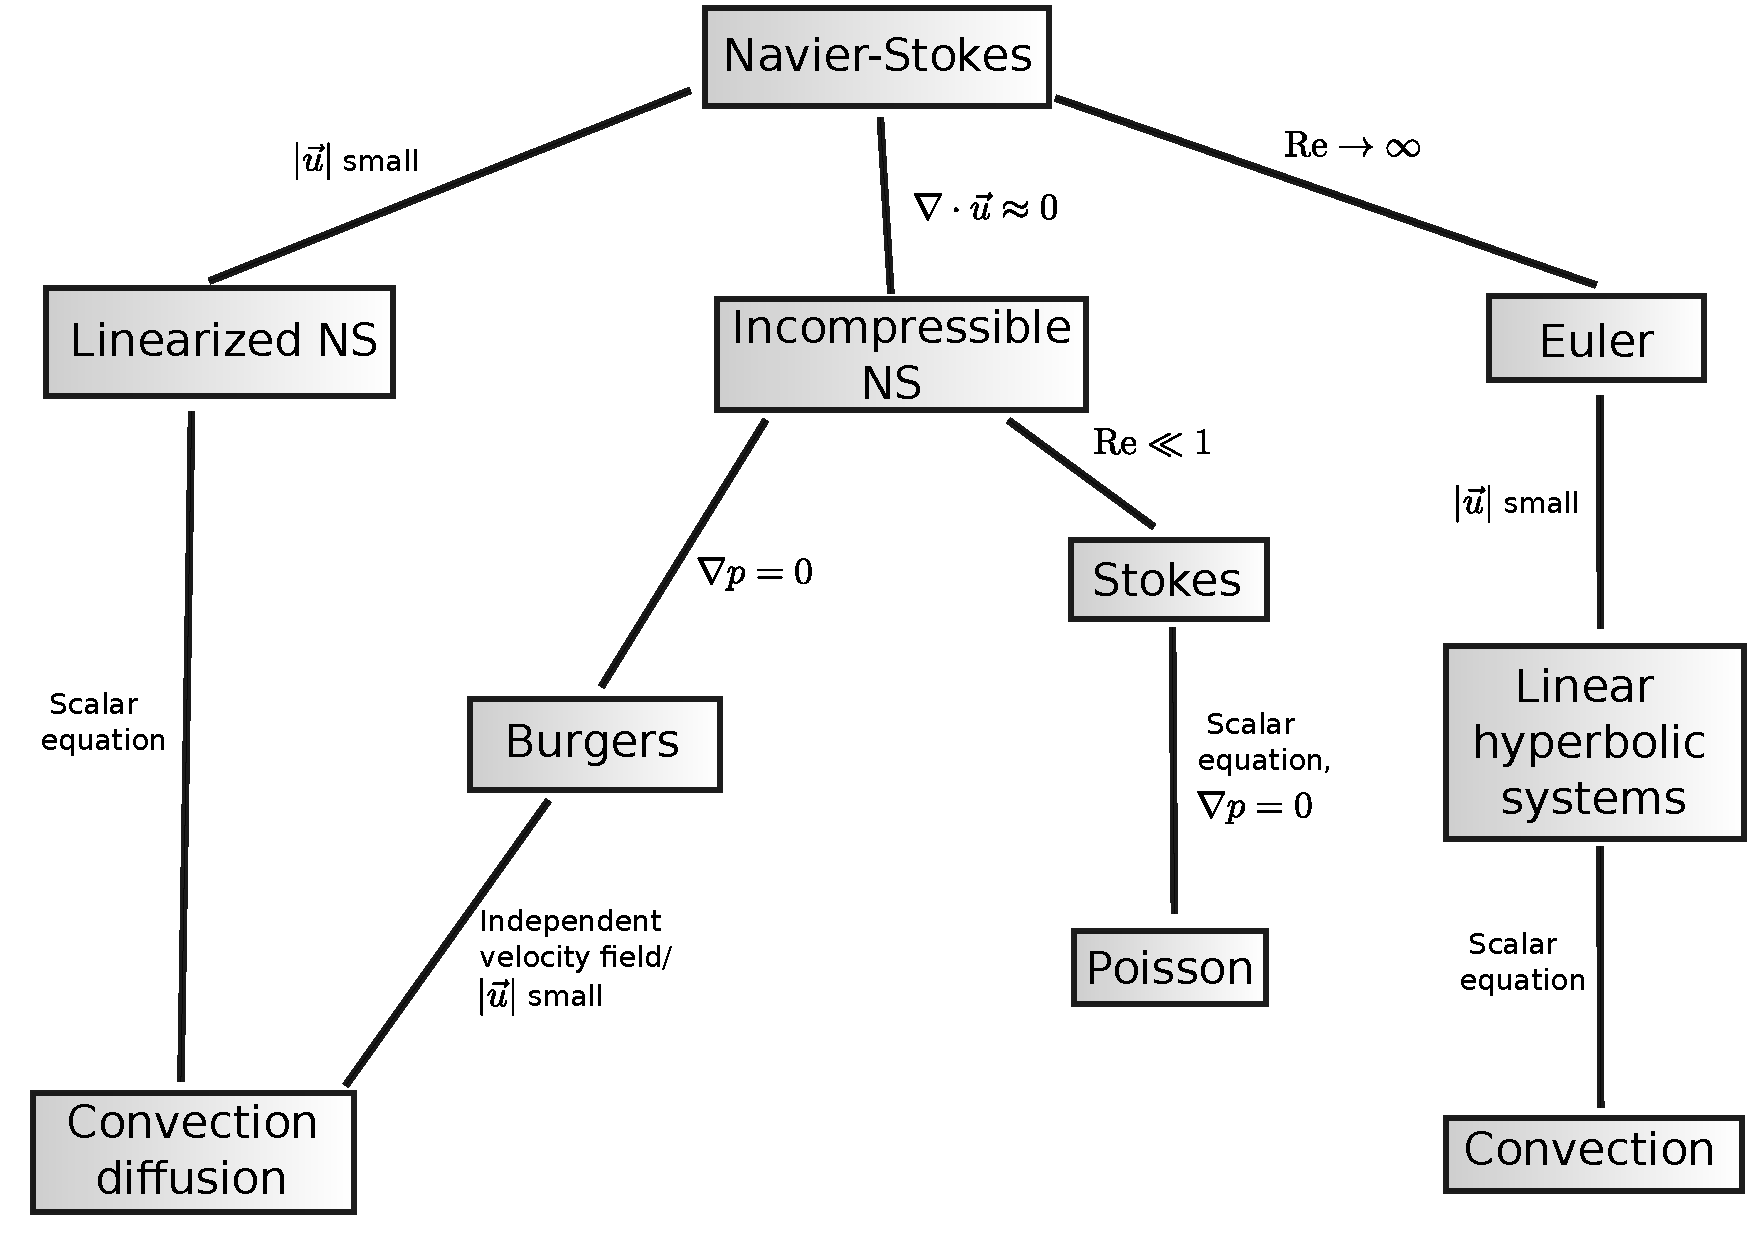
\includegraphics[scale=.45]{figs/CFD_tree.pdf}
\caption{A diagram of common CFD problems and their simplifying assumptions.}
\end{figure}

\section{The compressible Navier-Stokes equations}
\seclab{sec:compNS}

We consider the transient compressible Navier-Stokes equations. For simplicity, we present them in two spatial dimensions. Each equation of the Navier-Stokes system represents the conservation of some physical quantity in the behavior of a fluid inside a general control volume.\footnote{The derivation of the compressible Navier-Stokes equations is a standard result of the Reynolds transport theorem, and can be found in many elementary fluid dynamics books. See \cite{Emanuel:994127} for one example.} 

In 2D, the classical form of the Navier-Stokes equations involve the fluid density $\rho$, velocity in the $x$ and $y$ directions $u$ and $v$ (or $u_1$ and $u_2$), respectively, temperature $T$, energy per unit mass $e$, and stress and heat flux vectors $\boldsymbol \sigma_i$ and $\vec{q}$. The equations are as follows:
\begin{itemize}
\item{\textbf{Mass conservation}}
\begin{align*}
\pd{\rho}{t} + \div \vecttwo{\rho u }{\rho v} &= 0
\end{align*}

\item{\textbf{Momentum conservation}}
\begin{align*}
\pd{\rho u_1}{t} + \div \left(\vecttwo{\rho u^2+p }{\rho u v} - \boldsymbol \sigma_{1}\right) &=0\\
\pd{\rho u_2}{t} + \div \left(\vecttwo{\rho u v}{\rho v^2+p } - \boldsymbol \sigma_{2}\right) &=0
\end{align*}

\item{\textbf{Energy conservation}}
\begin{align*}
\pd{\rho e}{t} + \div \left(\vecttwo{((\rho e)+p)u}{((\rho e)+p)v} - \boldsymbol \sigma_1 \cdot \boldsymbol u- \boldsymbol \sigma_2 \cdot \boldsymbol u + \vec{q}\right) &=0
\end{align*}
\end{itemize}

We assume our fluid satisfies standard stress laws for $\boldsymbol \sigma$ and $\boldsymbol q$ as well. For viscous stresses $\boldsymbol \sigma$, we assume a Newtonian fluid
\begin{align*}
\sigma_{ij} &= \mu(u_{i,j}+u_{j,i}) + \lambda u_{k,k}\delta_{ij}.
\end{align*}
The coefficients $\lambda$ and $\mu$ are the viscosity and bulk viscosity, respectively. The bulk viscosity is often set implicitly through $2\mu + 3\lambda = 0$, known as Stokes' hypothesis. However, since the effect of bulk viscosity can become important for compressible flows, we treat both coefficients separately. In general, $\mu$ and $\lambda$ are functions of temperature, obeying the power law
\[
\mu = \left(\frac{T}{T_0}\right)^\beta,
\]
where $T_0$ is a reference temperature. We choose $\beta = 2/3$ in this case. 

We assume our fluid satisfies Fourier's law, which relates the heat flux $\boldsymbol q$ to the gradient of the temperature through
\begin{align*}
{\boldsymbol q} &= \kappa \grad T,
\end{align*}
where $\kappa$, the coefficient of heat conductivity, is generally a function of temperature. 

Finally, we assume our fluid is a thermally and calorically perfect ideal gas. Let $c_p$ and $c_v$ be the specific heats at constant pressure and volume, respectively. Then,
\begin{align*}
p &= (\gamma-1)\rho\iota\\
\iota &= e-\frac{1}{2}(u_1^2+u_2^2)\\
\iota &= c_vT
\end{align*}
where $e$ and $\iota$ are energy and internal energy per unit mass, respectively. 

As mentioned before, the compressible Navier-Stokes equations are especially of interest in the simulation of high-speed air flows. In other contexts, however, the compressible Navier-Stokes equations may be simplified based on physical assumptions about the problem at hand. We briefly cover several simplifying assumptions common in CFD applications. 

\subsection{Incompressibility}

Under appropriate assumptions on the behavior of density and temperature, the behavior of the compressible Navier-Stokes equations can be sufficiently represented by the incompressible Navier-Stokes equations for some fluid flows.  For example, the incompressible Navier-Stokes equations accurately model nearly incompressible mediums such as water, as well as low Mach number flows of compressible fluids. The study of the incompressible Navier-Stokes equations is an open area in mathematics, and is one of the most famous Millenium Problems posed by the Clay Mathematics Institute. The equations of incompressible flow pose a difficult problem computationally as well, in part due to the problem of the simulation of turbulent phenomena. 

For highly viscous ``creeping'' flows, the incompressible Navier-Stokes equations reduce down to the Stokes equations. We remark that determining good finite element spaces for the Stokes problem is still an active area of research. \cite{stokesFEM} lists several choices of finite element discretizations suitable for the Stokes equation. 

The scope of this dissertation will not deal with these two equations --- the Stokes equations are treated in \cite{stokesDPG}, and the incompressible Navier-Stokes are covered in an upcoming dissertation. 

\subsection{The linearized Navier-Stokes equations}

The linearized Navier-Stokes equations are the result of small perturbation assumptions applied to the full Navier-Stokes equations. Under such assumptions, the flow in a domain consists only of slight variations (to a given background flow) that are small compared to the magnitude of the free stream velocity.  Mathematically speaking, the linearized Navier-Stokes equations are the results of the linearization of the full equations with respect to a specific background flow.  The linearized NS equations are frequently referred to as an ``acoustic problem'', as they are used to study sound propagation.  

We are interested in the linearized Navier-Stokes equations mainly for mathematical purposes - as the solution to the full Navier-Stokes equations involves a series of solutions for linearized Navier-Stokes, we wish to investigate the behavior of our numerical method with respect to this system.  

\section{The scalar convection-diffusion equation}

Recall that the scalar convection-diffusion equation models mathematically the distribution of the concentration $u$ of a substance in a medium due to both convective and diffusive effects. 
%The general form of the equation in $\mathbb{R}^n$ is 
%\[
%\beta\cdot \grad u - \epsilon \Delta u = f,
%\]
%where $\beta \in \mathbb{R}^n$ is a vector specifying the direction of convection.
Scalar convection-diffusion has significant historical importance, as it is the prototypical model problem for solving the full Navier-Stokes equations --- most stabilized methods consider first the scalar convection-diffusion equation as a test case before attempting a solution of the full Navier-Stokes equations. As discussed previously, an important feature of the convection-diffusion equation is that solutions can develop boundary layers whose thickness depends on the viscosity, a physical feature found in most applications of interest for compressible flow. 

\subsection{Burgers' equation}

The Burgers' equation is physically derived from the incompressible Navier-Stokes equations under the assumption that $\grad p \approx 0$, or that the pressure field is near constant. A feature of the Burgers' equation not present in convection-diffusion is that, due to the presence of the nonlinear term, it can develop shock discontinuities in its solutions in finite time.  The Burgers' equation has also been used to study the phenomenon of turbulence; however, the Burgers equation does not exhibit the chaotic nature and sensitivity to initial conditions that characterizes turbulence as observed in the full and incompressible Navier-Stokes equations. 

The Burgers' equation is also the simplest nonlinear extension of the linear convection-diffusion equation, and exact solutions can sometimes be found using the method of characteristics. In the scope of this dissertation proposal, Burgers shall be used as to test the extension of our numerical method to nonlinear problems. 

\section{The inviscid case}

The pure convection equation is a result of neglecting the viscous term in the convection-diffusion equation. Physically speaking, these assumptions correspond to the inviscid limit, as well as a particular class of boundary conditions (for example, a prescribed inflow condition may be incompatible with the wall boundary condition $u = 0$ in the inviscid limit).  The Euler equations are likewise a result of neglecting the viscous terms in the Navier-Stokes equations.  However, these problems can be ill-posed in the continuous setting.  Take, for example, the vortex problem in Figure~\ref{fig:convCirc}.  A feature of the convection equation is that there is no crosswind diffusion - thus, materials do not mix across streamlines.  However, for the vortex problem, this also implies that the solution on any closed streamline can take any arbitrary value, and is thus undefined. 

\begin{figure}[!h]
\centering
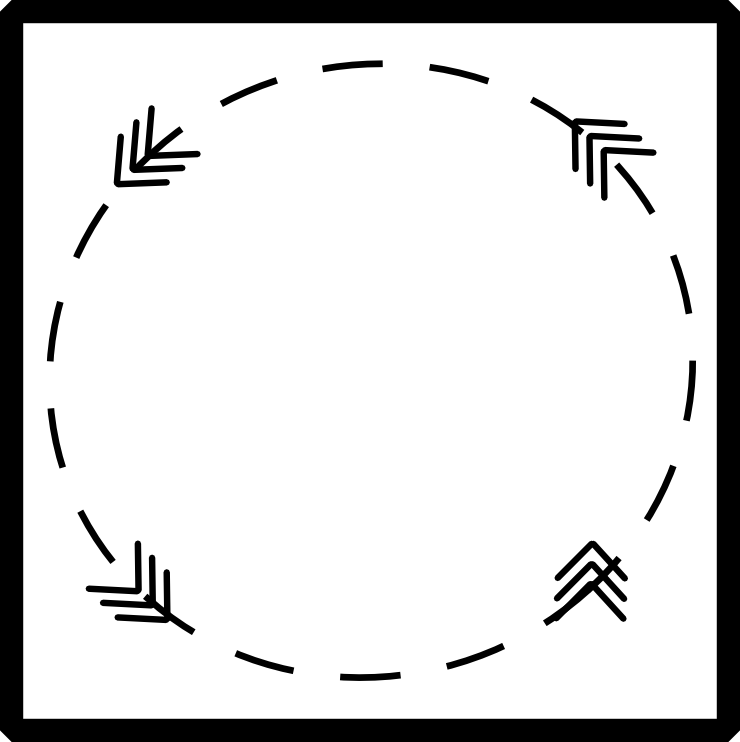
\includegraphics[scale = .22]{figs/convCirc.png}
\caption{Setup for the vortex problem.}
\label{fig:convCirc}
\end{figure}
Formally speaking, the solution to the vortex problem is taken to be the solution to the convection-diffusion equation (with appropriate outflow boundary conditions) as the viscosity tends towards zero, in which case, the solution in the interior would be uniformly zero (this technique is referred to in mathematical literature as the ``vanishing viscosity" method, and is used to define unique solutions in the inviscid limit).  This motivates the need for \emph{artificial viscosity} methods with which to regularize inviscid solutions.  The topic is expansive, and we direct the reader towards \cite{Barter} for a more detailed discussion of past and present artificial viscosity methods. 

The full Navier-Stokes models have proven difficult to solve due to the mathematical nature of the equations --- due to the lack of robustness of most methods, solving the Navier-Stokes for high Reynolds numbers requires very fine meshes and is an incredibly expensive task.  Additionally, the problem of turbulence for high Reynolds numbers further complicates the Navier-Stokes solutions for high speed compressible flow.  Without turbulence models, turbulent effects can prevent convergence to a solution.  However, common turbulence models, such as Reynolds Averaged Navier-Stokes (RANS), can lead to nonphysical solutions, such as the existence of a steady-state solution when there is none.  

In comparison, the coupling of the inviscid Euler equations with boundary layer models has been successful in simulating many phenomena in compressible flow at a computational cost orders of magnitude below that of the full Navier-Stokes equations \cite{BoeingDrela}.  The method has been extended to a wide array of physical conditions, and is an active area of current research in both industry and academia.  
